\section*{Тестирование программы}

Запустим программу.

На экране появится справка по командам и 
приглашение к вводу (рис.\ref{test.start}).

\begin{figure}[H]
    \centering
    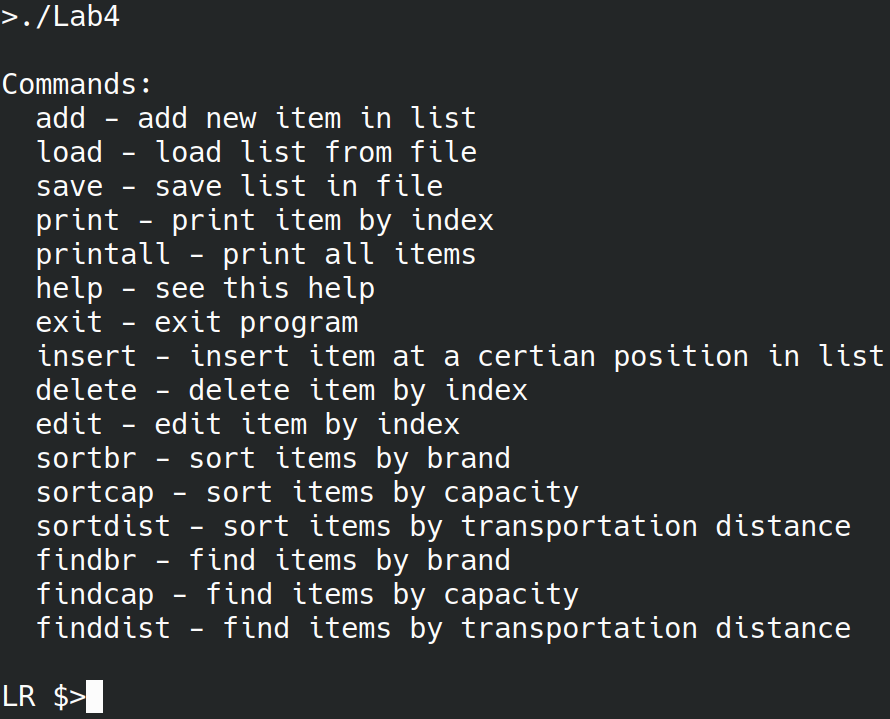
\includegraphics[width=0.9\linewidth]{photo/test.start}
    \caption{Начало работы}
    \label{test.start}
\end{figure}

Введём случайное слово. 
Программа не распознает комманду и предложит 
использовать 'help' (рис.\ref{test.unknown_command}). 

\begin{figure}[H]
    \centering
    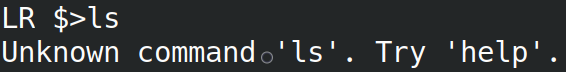
\includegraphics[width=0.9\linewidth]{photo/test.unknown_command}
    \caption{Неизвестная команда}
    \label{test.unknown_command}
\end{figure}

Введём команду 'help', чтобы получить справку (рис.\ref{test.help}).

\begin{figure}[H]
    \centering
    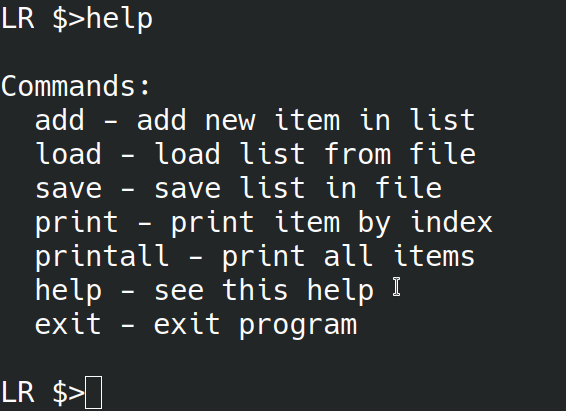
\includegraphics[width=0.9\linewidth]{photo/test.help}
    \caption{Справка}
    \label{test.help}
\end{figure}

На попытки распечатать элементы пустого списка
программа отвечает, что нечего печатать и предлагает
использовать команду 'add' (рис.\ref{test.print_empty}).

\begin{figure}[H]
    \centering
    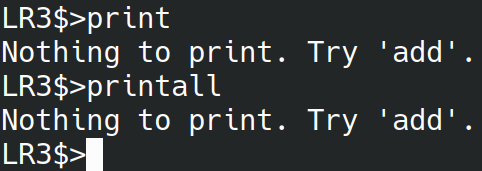
\includegraphics[width=0.9\linewidth]{photo/test.print_empty}
    \caption{Печть пустого списка}
    \label{test.print_empty}
\end{figure}

Добавим 2 элемента в список, используя 'add'(рис.\ref{test.add},\ref{test.add2}).
В случае попытки ввести некорректные данные 
ввод зацикливается (рис.\ref{test.add}) до тех пор,
пока не будут введены корректные данные.

\begin{figure}[H]
    \centering
    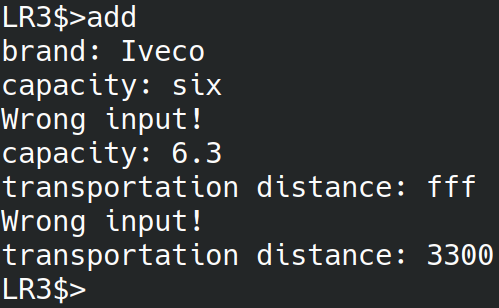
\includegraphics[width=0.9\linewidth]{photo/test.add}
    \caption{Добавление 1 элемента в список}
    \label{test.add}
\end{figure}

\begin{figure}[H]
    \centering
    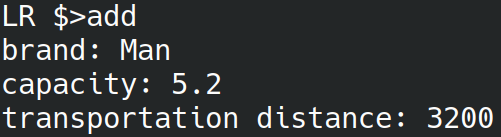
\includegraphics[width=0.9\linewidth]{photo/test.add2}
    \caption{Добавление 2 элемента в список}
    \label{test.add2}
\end{figure}

Распечатаем первый элемент (с индексом 0) с помощью команды 'print' (рис.\ref{test.print0}).

\begin{figure}[H]
    \centering
    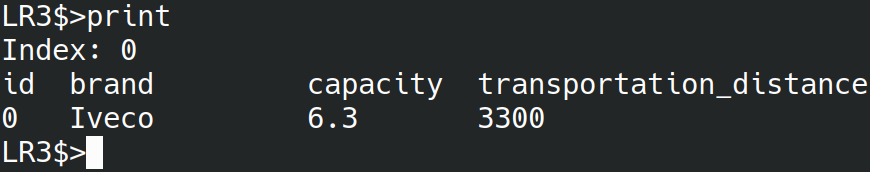
\includegraphics[width=0.9\linewidth]{photo/test.print0}
    \caption{Вывод первого элемента}
    \label{test.print0}
\end{figure}

Распечатаем все элементы списка с помощью команды 'printall' (рис.\ref{test.printall}).

\begin{figure}[H]
    \centering
    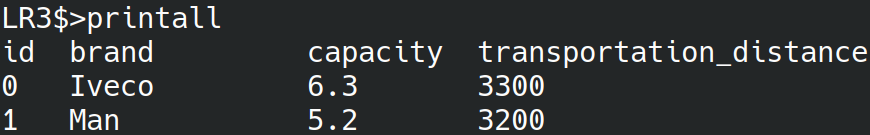
\includegraphics[width=0.9\linewidth]{photo/test.printall}
    \caption{Вывод элементов списка}
    \label{test.printall}
\end{figure}

Сохраним текущий список.

Если попытаться передать директорию, программа не сохранит файл (рис.\ref{test.save.dir}).

\begin{figure}[H]
    \centering
    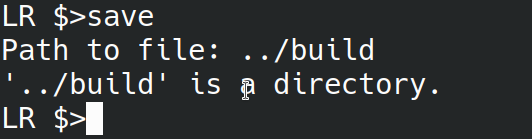
\includegraphics[width=0.9\linewidth]{photo/test.save.dir}
    \caption{Сохранение файла под именем директории}
    \label{test.save.dir}
\end{figure}

Если попытаться перезаписать существующий файл, программа попросит подтверждение.

Можно отказаться (рис.\ref{test.save.n}).

\begin{figure}[H]
    \centering
    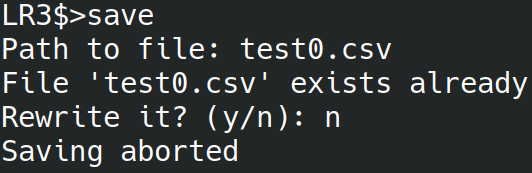
\includegraphics[width=0.9\linewidth]{photo/test.save.n}
    \caption{Отказ от перезаписи}
    \label{test.save.n}
\end{figure}

Можно согласиться (рис.\ref{test.save.y}).

\begin{figure}[H]
    \centering
    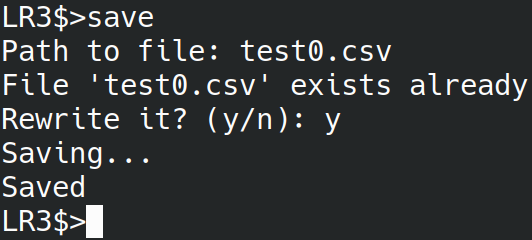
\includegraphics[width=0.9\linewidth]{photo/test.save.y}
    \caption{Соглашение на перезапись}
    \label{test.save.y}
\end{figure}

Сохранённый файл виден на рис.\ref{test.file}.

\begin{figure}[H]
    \centering
    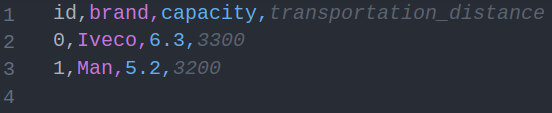
\includegraphics[width=0.9\linewidth]{photo/test.file}
    \caption{Сохранённый файл}
    \label{test.file}
\end{figure}

При загрузке файла программа выдаст предупреждение, что 
загрузка перезапишет текущий список, и попросит подтверждение (рис.\ref{test.load.exist})

\begin{figure}[H]
    \centering
    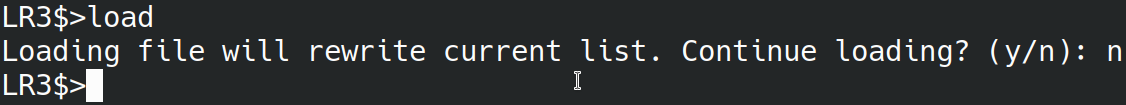
\includegraphics[width=0.9\linewidth]{photo/test.load.exist}
    \caption{Предупреждение при загрузке файла}
    \label{test.load.exist}
\end{figure}

Перезапустим программу, чтобы очистить список.

Попытаемся загрузить файл (рис.\ref{test.file}) с помощью команды 'load'.

При попытке передачи директории или несуществующего файла, 
программа предупредит об этом и остановит загрузку.
Загрузим файл и проверим, что данные считались корректно 
с помощью команды 'printall' (рис.\ref{test.load}).

\begin{figure}[H]
    \centering
    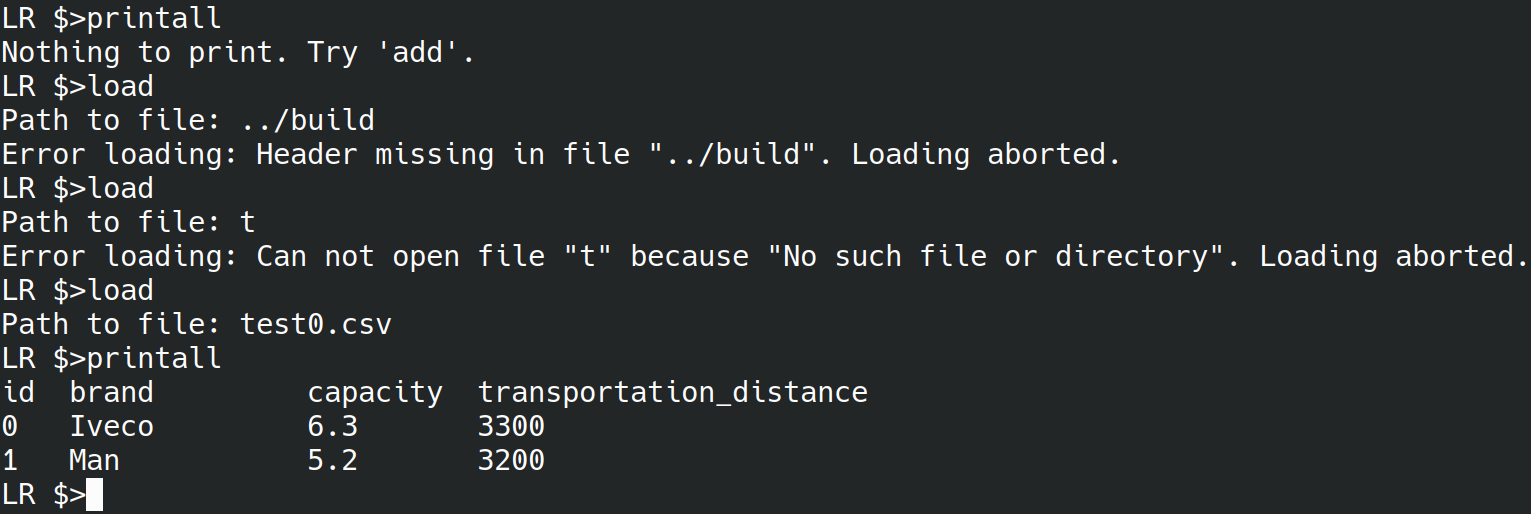
\includegraphics[width=0.9\linewidth]{photo/test.load}
    \caption{Загрузка файла}
    \label{test.load}
\end{figure}

Перезапустим программу ещё раз, чтобы очистить список.

При применении комманд
'edit',
'delete', или
'insert'
на пустом списке программа будет выдавать сообщение 
о том, что список пуст.
При применении комманд
'sortbr',
'sortcap', или
'sortdist'
на пустом списке программа не будет реагировать.
При применении комманд
'findbr',
'findcap', или
'finddist'
на пустом списке программа будет выдавать нулевой 
результат поиска при любых
входных данных (рис.\ref{test.empty}).

\begin{figure}[H]
    \centering
    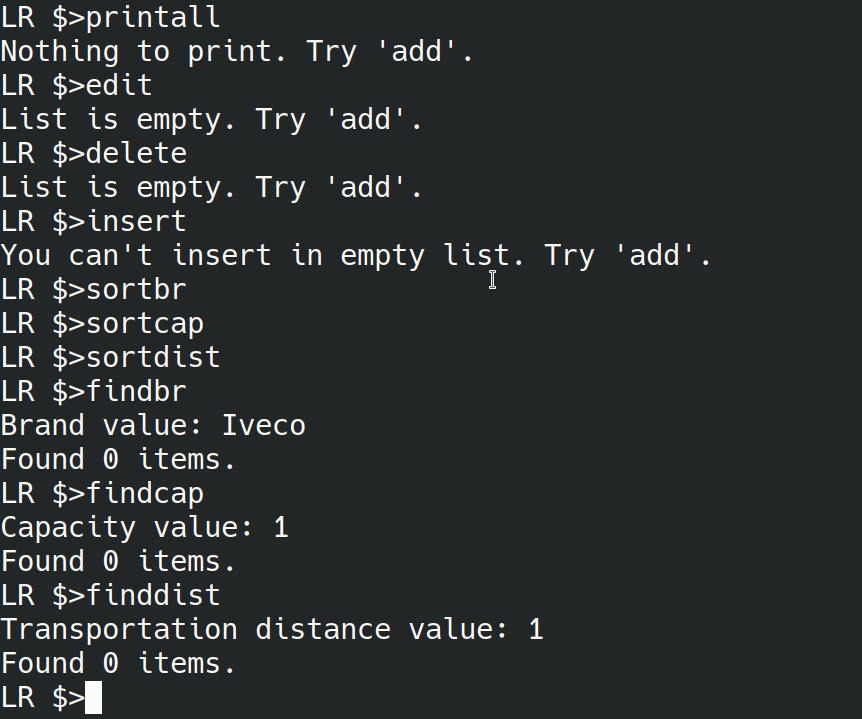
\includegraphics[width=0.9\linewidth]{photo/test.empty}
    \caption{Применение команд на пустом списке}
    \label{test.empty}
\end{figure}

Загрузим список из подготовленного файла (рис.\ref{test.bigfile1}).

\begin{figure}[H]
    \centering
    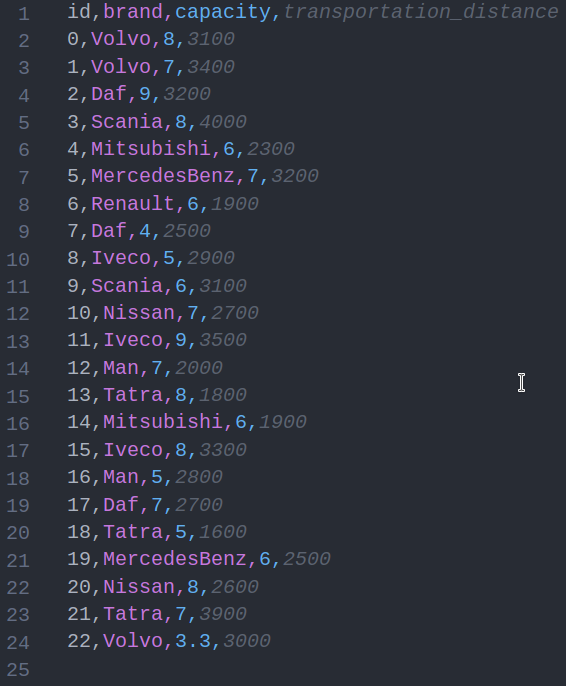
\includegraphics[width=0.9\linewidth]{photo/test.bigfile1}
    \caption{Загружаемый файл}
    \label{test.bigfile1}
\end{figure}

Загруженный файл распечетаем с 
помощью команды 'printall' (рис.\ref{test.bigload}).

\begin{figure}[H]
    \centering
    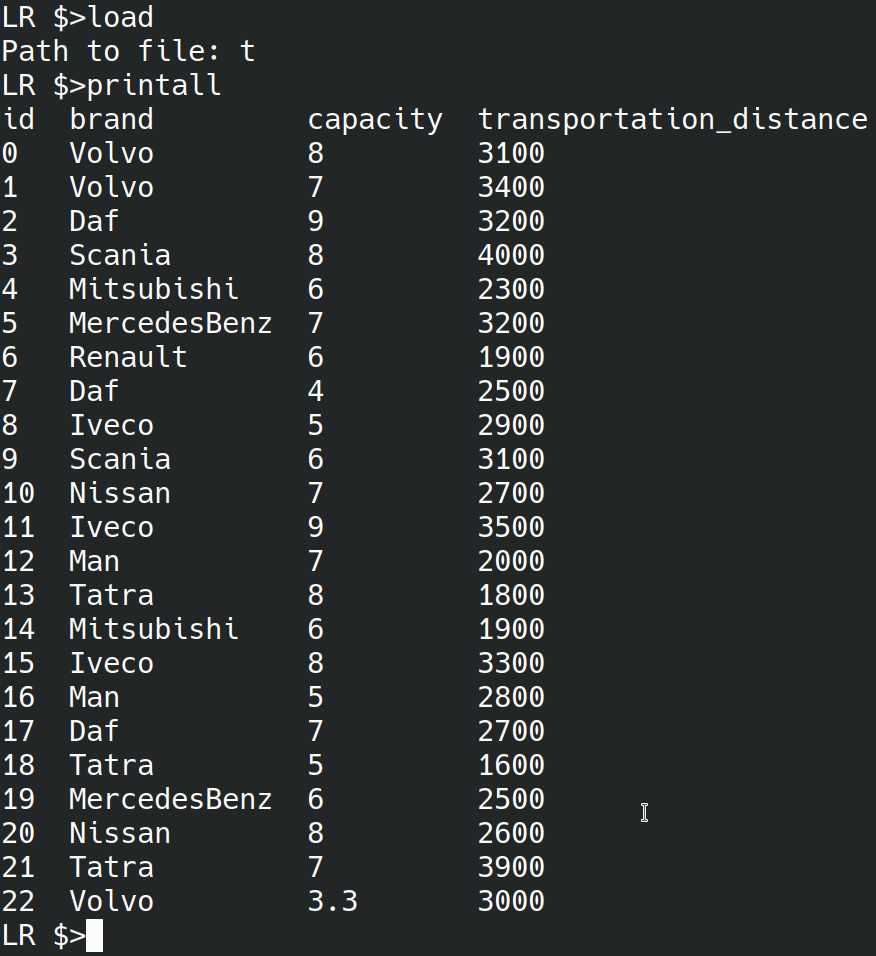
\includegraphics[width=0.9\linewidth]{photo/test.bigload}
    \caption{Загрузка файла}
    \label{test.bigload}
\end{figure}

Выполним команду 'edit' над элементом 22, изменив 
марку на 'Man',
грузоподъёмность на 5.2,
дальность перевозки на 2700,
после распечатаем элемент с помощью команды 'print'.
(рис.\ref{test.edit})

\begin{figure}[H]
    \centering
    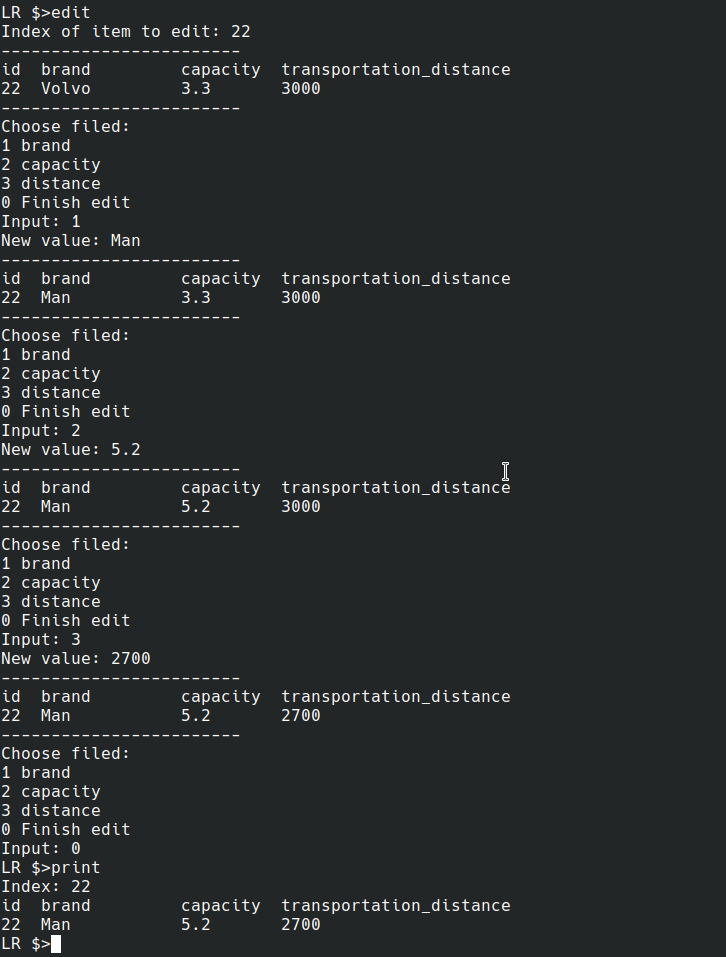
\includegraphics[width=0.9\linewidth]{photo/test.edit}
    \caption{Редактирование элемента}
    \label{test.edit}
\end{figure}

Выполним команду 'insert' и вставим новый элемент
перед элементом с индексом 4, установив значения всех
полей в '1' (рис.\ref{test.insert}). 

\begin{figure}[H]
    \centering
    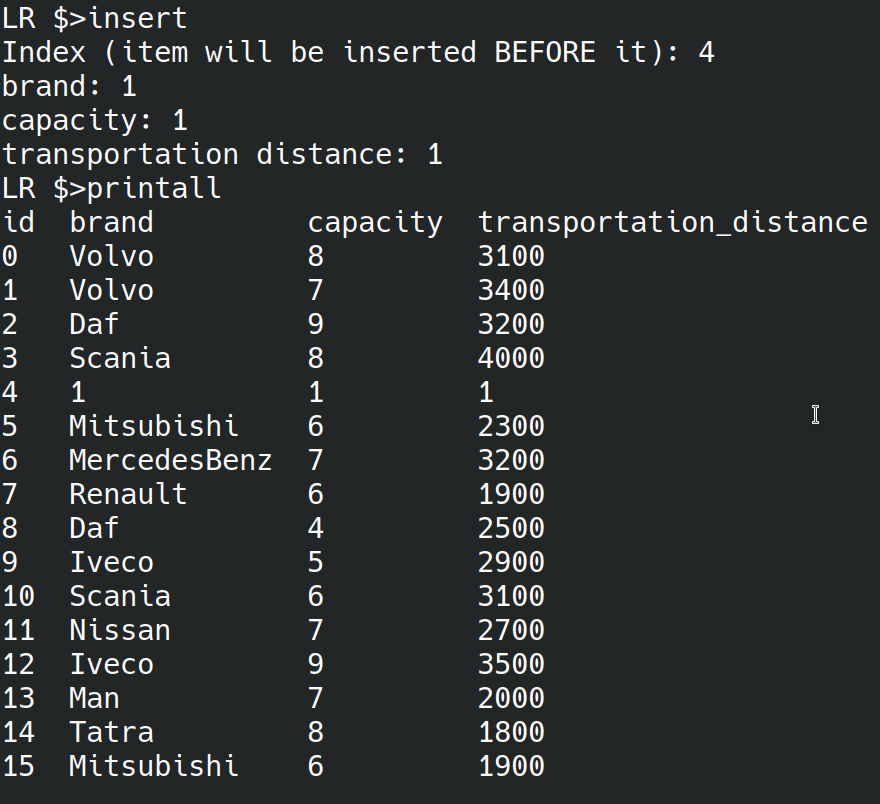
\includegraphics[width=0.9\linewidth]{photo/test.insert}
    \caption{Вставка элемента}
    \label{test.insert}
\end{figure}

Выполним команду 'delete', чтобы удалить только что вставленный элемент
(рис.\ref{test.delete}).

\begin{figure}[H]
    \centering
    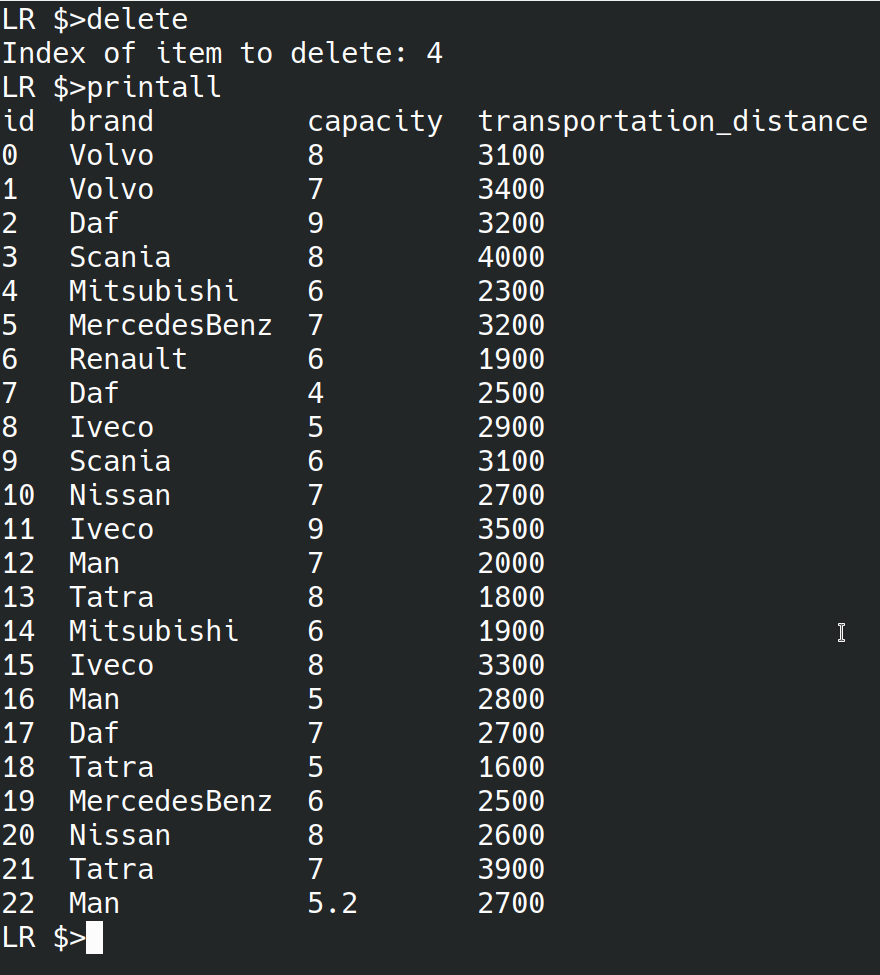
\includegraphics[width=0.9\linewidth]{photo/test.delete}
    \caption{Удаление элемента}
    \label{test.delete}
\end{figure}

Выполним команду 'sortbr', чтобы отсортировать 
список по марке (в лексиграфическом порядке)(рис.\ref{test.sortbr}).

\begin{figure}[H]
    \centering
    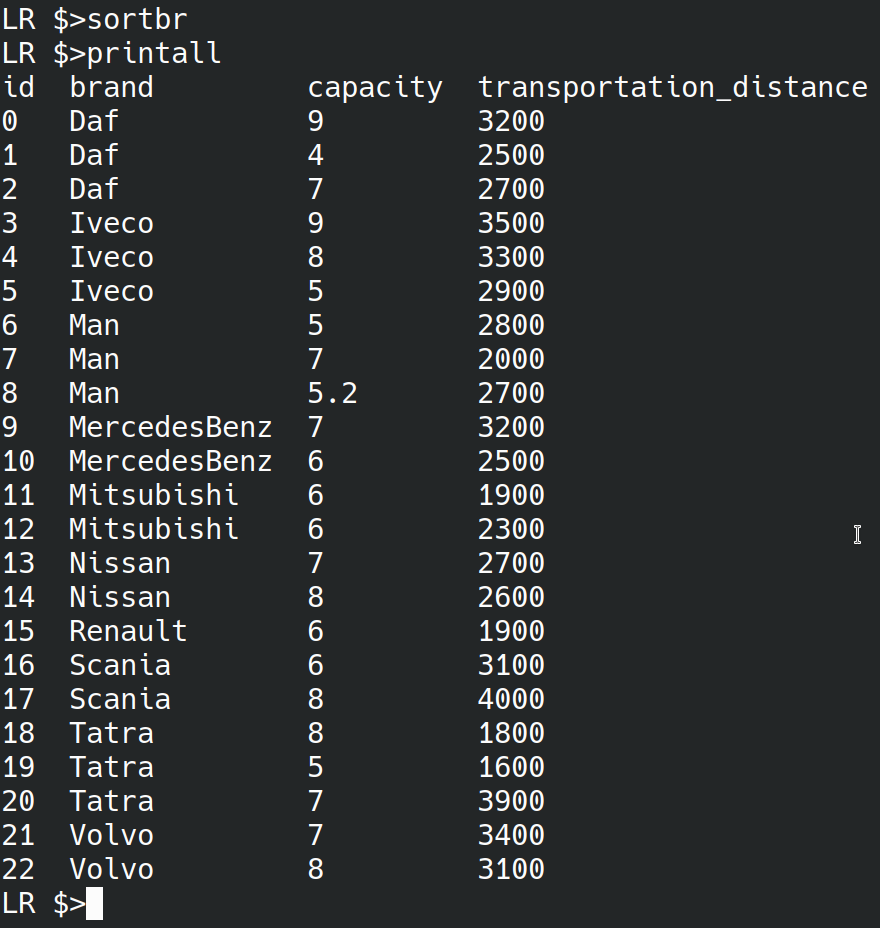
\includegraphics[width=0.9\linewidth]{photo/test.sortbr}
    \caption{Сортировка по марке}
    \label{test.sortbr}
\end{figure}

Выполним команду 'sortcap', чтобы отсортировать 
список по грузоподъёмности (по возрастанию)(рис.\ref{test.sortcap}).

\begin{figure}[H]
    \centering
    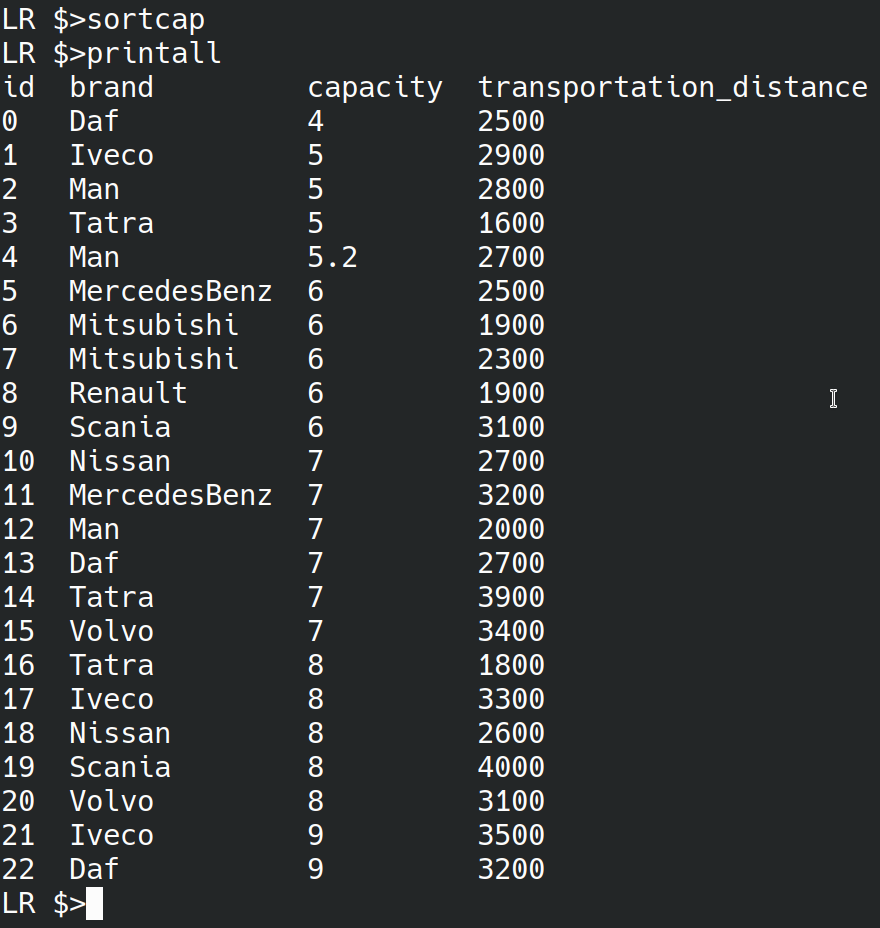
\includegraphics[width=0.9\linewidth]{photo/test.sortcap}
    \caption{Сортировка по грузоподъёмности}
    \label{test.sortcap}
\end{figure}

Выполним команду 'sortdist', чтобы отсортировать 
список по дальности перевозки (по возрастанию)(рис.\ref{test.sortdist}).

\begin{figure}[H]
    \centering
    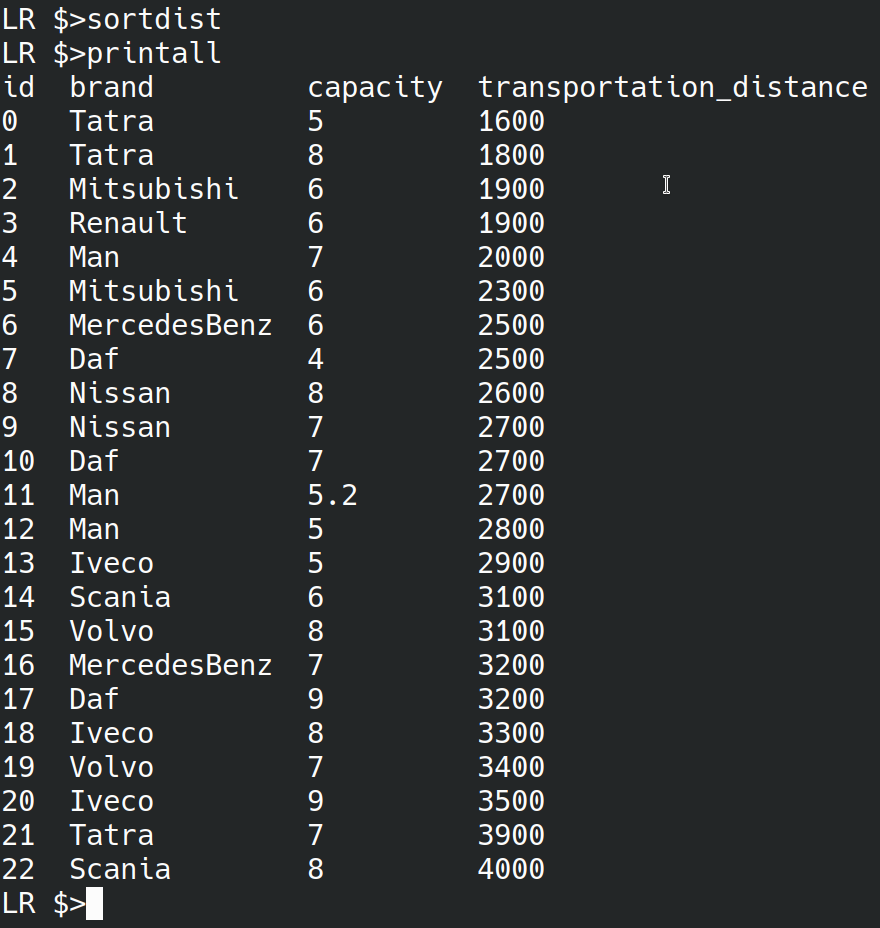
\includegraphics[width=0.9\linewidth]{photo/test.sortdist}
    \caption{Сортировка по дальности перевозки}
    \label{test.sortdist}
\end{figure}

Выполним команду 'findbr', чтобы найти все элементы с
маркой 'Tatra' (рис.\ref{test.findbr}).

\begin{figure}[H]
    \centering
    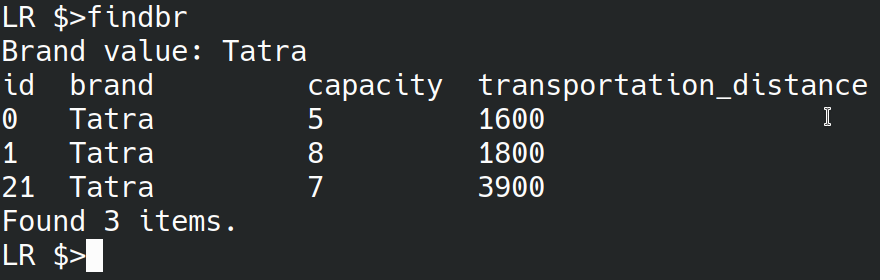
\includegraphics[width=0.9\linewidth]{photo/test.findbr}
    \caption{Поиск по марке}
    \label{test.findbr}
\end{figure}

Выполним команду 'findcap', чтобы найти все элементы с
грузоподъёмностью '7' (рис.\ref{test.findcap}).

\begin{figure}[H]
    \centering
    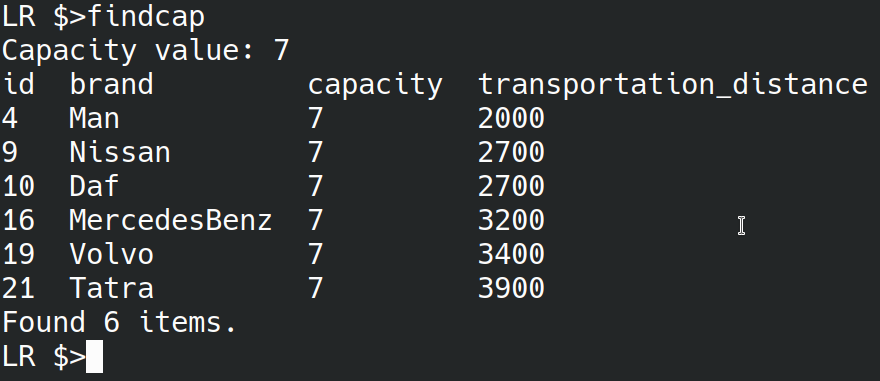
\includegraphics[width=0.9\linewidth]{photo/test.findcap}
    \caption{Поиск по грузоподъёмности}
    \label{test.findcap}
\end{figure}

Выполним команду 'finddist', чтобы найти все элементы с
дальностю перевозки '2700' (рис.\ref{test.finddist}).

\begin{figure}[H]
    \centering
    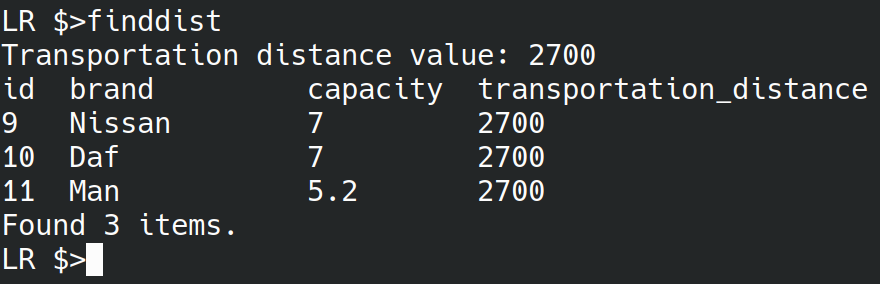
\includegraphics[width=0.9\linewidth]{photo/test.finddist}
    \caption{Поиск по дальности перевозки}
    \label{test.finddist}
\end{figure}

Выполним команду 'exit', чтобы выйти из программы (рис.\ref{test.exit}).

\begin{figure}[H]
	\centering
	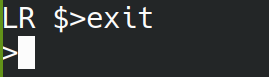
\includegraphics[width=0.35\linewidth]{photo/test.exit}
	\caption{Выход из программы}
	\label{test.exit}
\end{figure}